\chapter{系统架构}

\section{桌面端架构}

\begin{figure}[H]
  \centering
  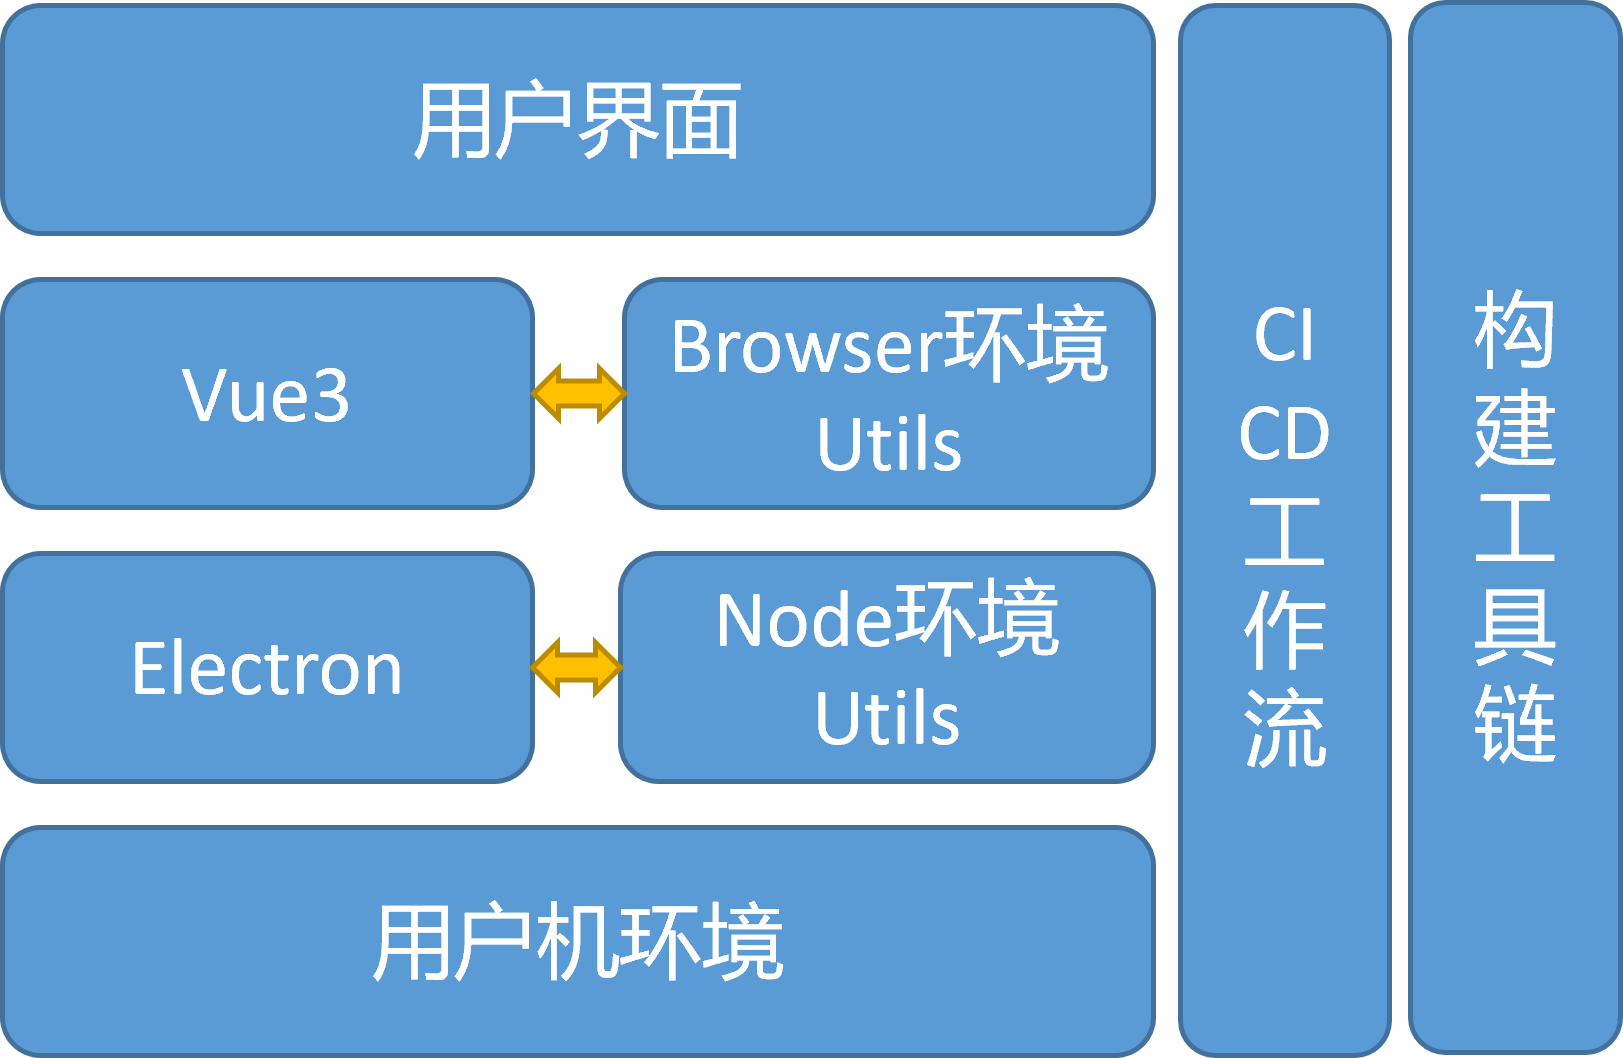
\includegraphics[scale=0.75]{figure/front_arch.png}
  \caption{\textbf{桌面端架构图}}
  \label{fig:front_arch}
\end{figure}

\figref{fig:front_arch}是PhoeniX的桌面端架构图。PhoeniX桌面端以TypeScript为主要编程语言,采用Vite和Electron-Builder作为构建工具链,使用Github Action作为核心CI/CD工作流。PhoeniX围绕Electron框架搭建,在Electron之上集成了Vue3,使用Electron与用户机进行必要的交互,而使用Vue3完成主要应用逻辑的编写。PhoeniX主要使用Naive-UI构建用户界面,另外还使用了Monaco等第三方组件,提供一致而流畅的用户体验。

\section{服务端架构}

\begin{figure}[H]
  \centering
  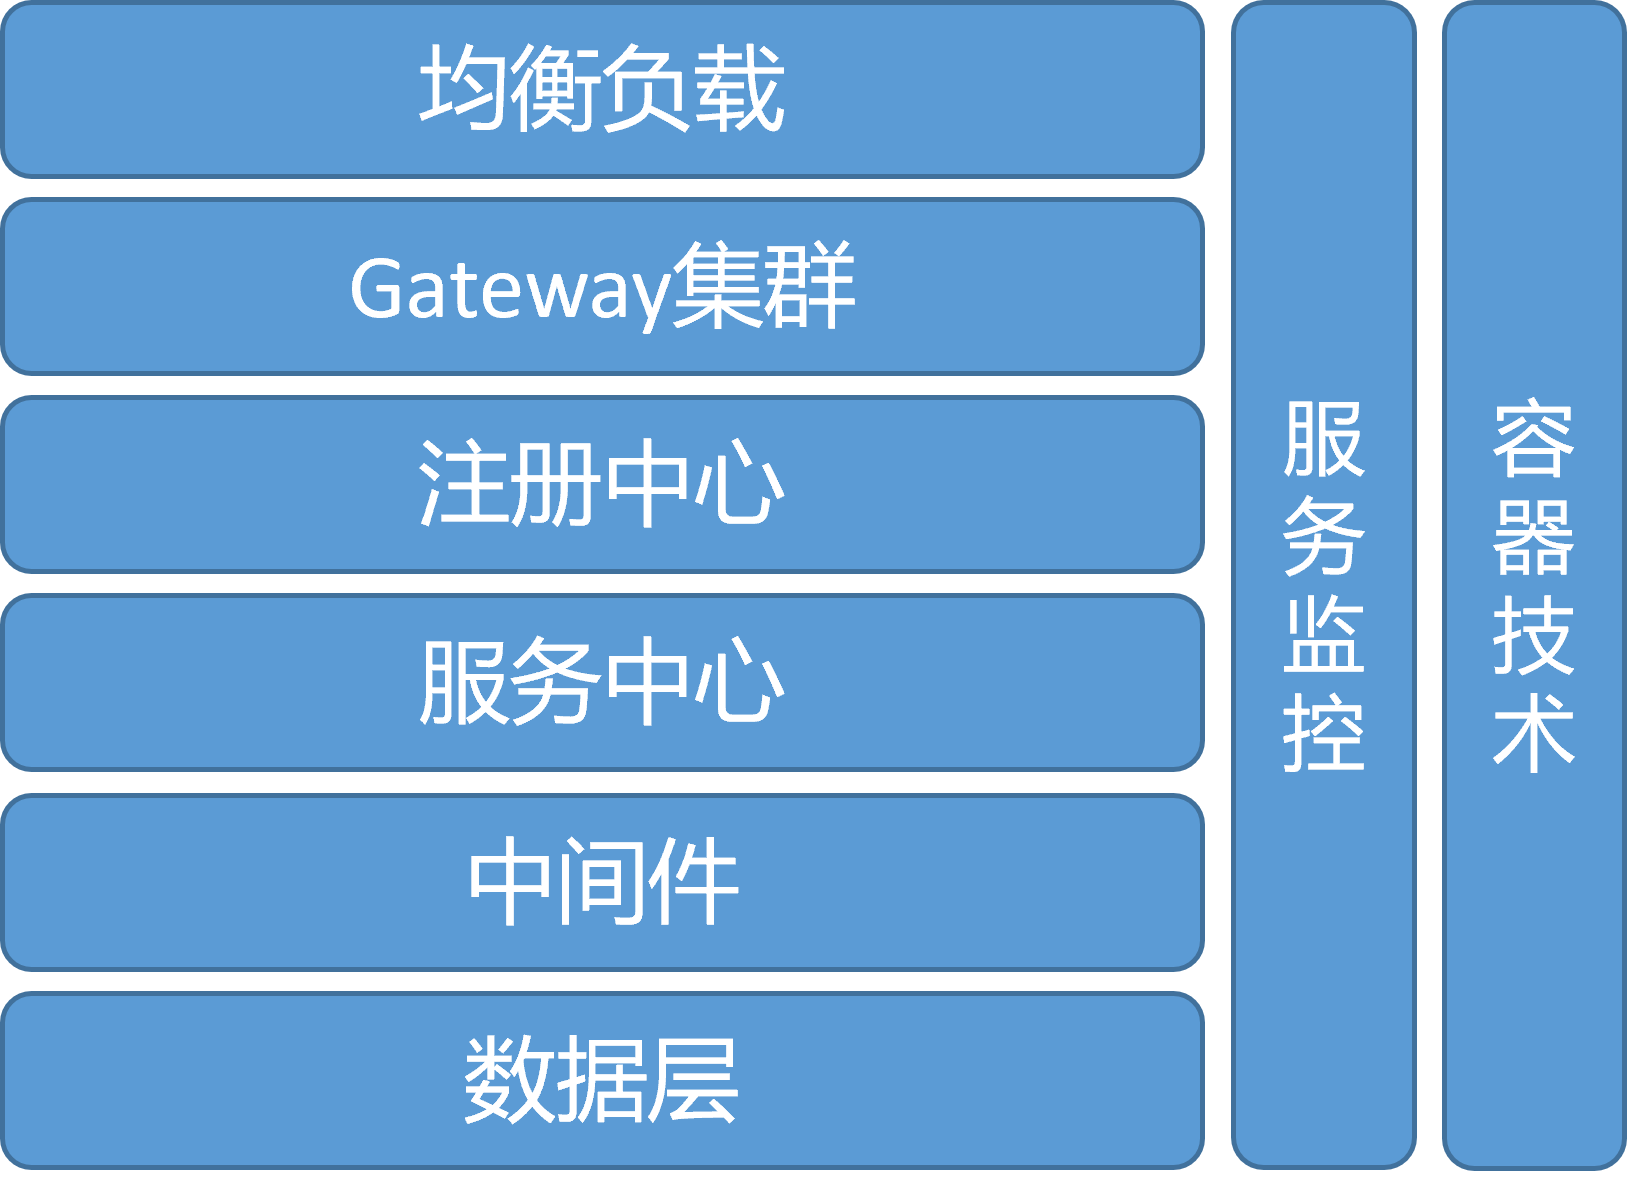
\includegraphics[scale=0.75]{figure/back_arch.png}
  \caption{\textbf{服务端架构图}}
  \label{fig:back_arch}
\end{figure}

\figref{fig:back_arch}是PhoeniX的服务端架构图。PhoeniX服务端采用微服务架构,以Golang为主要编程语言,采用Kubernetes作为服务端的运维基础,使用Prometheus对部署的各个服务进行监控。PhoeniX的服务端能够支撑高并发请求,用户流量到达服务端时,首先会到达LVS均衡负载层,均衡负载层会将请求分流到网关(Gateway)集群中的各个服务器。网关服务器提供聚合服务、路由等功能,流量经过网关服务器后到到Etcd注册中心,随后分发给对应的微服务。各个微服务采用Gin框架编写核心逻辑,使用gRPC作为RPC框架。服务中心请求数据时,将请求发送到消息中间件RabbitMQ中,不直接从MySQL等数据库中读取数据,起到流量削峰的作用。